\chapter{Assignment 2 --- Rotation Matrices}
\label{ch:hw2}

% cleveref names follow the language of the surrounding prose.
\crefname{equation}{식}{식}
\Crefname{equation}{식}{식}
\crefname{figure}{그림}{그림}
\Crefname{figure}{그림}{그림}
\crefname{table}{표}{표}
\Crefname{table}{표}{표}
\crefname{section}{절}{절}
\Crefname{section}{절}{절}
\crefname{chapter}{장}{장}
\Crefname{chapter}{장}{장}

\section{배경 --- 회전 행렬은 무엇이고 왜 필요한가}
\label{sec:hw2-bg}

과제는 행렬을 주고 곱하라고만 한다. 이 절은 그 행렬이 어디에서 왔고 왜 필요한지를
정리한다. 이후 절들은 모두 영어로 되어 있다.

\subsection{왜 필요한가 --- 좌표계가 여러 개다}
\label{sec:hw2-bg-why}

로봇은 좌표계(frame)를 하나만 쓰지 않는다. 월드 좌표계, 로봇 베이스 좌표계, 관절마다
하나씩, 카메라 좌표계, 그리퍼 좌표계가 동시에 존재한다. 공간의 \emph{같은 한 점}이
좌표계마다 \emph{다른 세 숫자}로 표현된다는 뜻이다. 카메라가 ``물체가 내 앞
0.5\,m''라고 말할 때, 팔을 움직이려면 그 값을 베이스 좌표계의 값으로 바꿔야 한다.

회전 행렬 $R$이 그 변환기다. 좌표계 사이의 \emph{방향(orientation)} 차이를 담당한다.
좌표계의 원점이 서로 떨어져 있는 경우, 즉 \emph{위치} 차이는 평행이동으로 따로
처리하며, 보통 회전과 평행이동을 하나로 묶은 $4 \times 4$ 동차 변환 행렬
(homogeneous transformation)을 쓴다. 이번 과제는 그중 회전 부분만 다룬다.

\subsection{두 가지 해석}
\label{sec:hw2-bg-two}

같은 행렬을 두 가지로 읽을 수 있고, 둘을 섞으면 부호에서 틀린다.

\begin{itemize}
  \item \textbf{능동적(active) 해석} --- 좌표계는 그대로 두고 \emph{벡터를} 돌린다.
        물체가 실제로 회전한 것이다.
  \item \textbf{수동적(passive) 해석} --- 벡터는 그대로 두고 \emph{좌표계를} 돌린 뒤
        같은 점을 새 좌표계에서 다시 표현한다. 이때 쓰는 행렬은 $R^{\mathsf{T}}$로,
        능동적 회전의 역이다.
\end{itemize}

이 장은 \textbf{능동적 해석}을 쓴다. $v_1$을 돌려서 $v_2$를 얻는다. 각도의 부호는
오른손 법칙을 따른다 --- 회전축의 양의 방향에서 원점을 내려다볼 때 반시계 방향이
양수다.

\subsection{어떻게 만들어지는가 --- 2차원에서의 유도}
\label{sec:hw2-bg-2d}

평면 위의 점 $(x, y)$를 원점 기준 극좌표로 쓴다. 반지름을 $r$, 시작 각도를 $\alpha$라
하면

\begin{equation}
\label{eq:hw2-bg-polar}
x = r\cos\alpha, \qquad y = r\sin\alpha .
\end{equation}

여기서 $\theta$만큼 더 돌리면 반지름은 그대로이고 각도만 $\alpha + \theta$가 된다
(\Cref{fig:hw2-bg-rot2d}). 삼각함수 덧셈정리를 적용하고
\Cref{eq:hw2-bg-polar}을 다시 대입하면

\begin{align}
x' &= r\cos(\alpha + \theta)
    = r\cos\alpha\cos\theta - r\sin\alpha\sin\theta
    = x\cos\theta - y\sin\theta, \label{eq:hw2-bg-xp} \\
y' &= r\sin(\alpha + \theta)
    = r\sin\alpha\cos\theta + r\cos\alpha\sin\theta
    = x\sin\theta + y\cos\theta. \label{eq:hw2-bg-yp}
\end{align}

행렬로 묶으면

\begin{equation}
\label{eq:hw2-bg-2d}
\begin{bmatrix} x' \\ y' \end{bmatrix}
=
\begin{bmatrix}
\cos\theta & -\sin\theta \\
\sin\theta & \cos\theta
\end{bmatrix}
\begin{bmatrix} x \\ y \end{bmatrix}.
\end{equation}

회전 행렬은 여기서 나온다. 새로 정의한 것이 아니라 덧셈정리를 행렬로 적은 것일
뿐이다.

\begin{figure}[ht]
% \caption's label is set by the class, not by cleveref - scoped to this
% figure so the English chapters keep "Figure".
\renewcommand{\figurename}{그림}
\centering
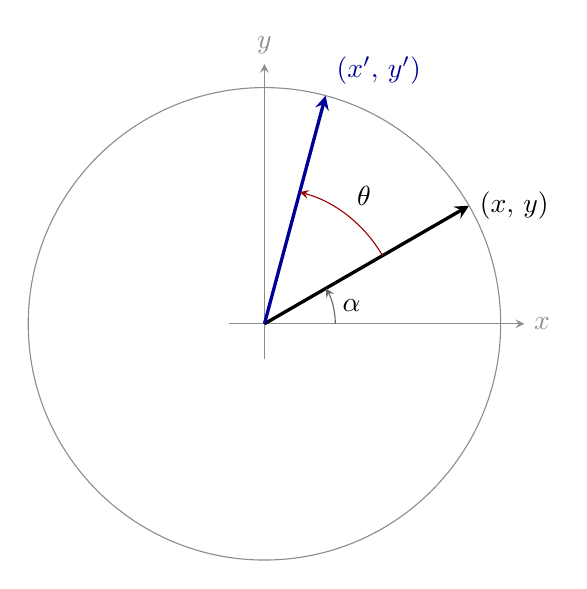
\begin{tikzpicture}[scale=1.5,>=stealth]
  \draw[->,black!45] (-0.3,0) -- (2.2,0) node[right] {$x$};
  \draw[->,black!45] (0,-0.3) -- (0,2.2) node[above] {$y$};
  \draw[->,very thick] (0,0) -- (1.732,1.0) node[right] {$(x,\,y)$};
  \draw[->,very thick,blue!60!black] (0,0) -- (0.518,1.932)
        node[above right] {$(x',\,y')$};
  \draw[black!45] (0,0) circle (2);
  \draw[->,red!60!black] (1.0,0.577) arc (30:75:1.155)
        node[midway,above right,black] {$\theta$};
  \draw[->,black!60] (0.6,0) arc (0:30:0.6) node[midway,right,black] {$\alpha$};
\end{tikzpicture}
\caption{2차원 회전. 반지름 $r$은 변하지 않고 각도만 $\alpha$에서
         $\alpha + \theta$로 늘어난다.}
\label{fig:hw2-bg-rot2d}
\end{figure}

\subsection{3차원으로 확장하기}
\label{sec:hw2-bg-3d}

어떤 축을 중심으로 돌리면 \emph{그 축 방향 성분은 변하지 않는다}. 그래서 3차원
회전 행렬은 \Cref{eq:hw2-bg-2d}의 $2 \times 2$ 블록을 나머지 두 좌표 자리에
끼워 넣고, 회전축 자리에는 1을 놓은 형태가 된다.

$Z$축 회전이 가장 직관적이다. $z$는 그대로이고 $(x, y)$가
\Cref{eq:hw2-bg-2d} 그대로 돌아간다 --- 그 결과가 \Cref{eq:hw2-rz}이다.
$X$축 회전도 같다. $x$는 그대로이고 $(y, z)$가 돌아간다
(\Cref{eq:hw2-rx}).

$Y$축 회전에서 부호가 뒤집혀 보이는 것이 늘 걸리는 부분이다. 이유는 순환 순서에
있다. 오른손 좌표계의 순환 순서는 $x \to y \to z \to x$이고, $Y$축을 뺀 나머지 쌍은
$(y, z)$나 $(x, y)$가 아니라 $(z, x)$다. 즉 \Cref{eq:hw2-bg-2d}에서
$x$ 자리에 $z$를, $y$ 자리에 $x$를 넣어야 한다.

\begin{equation}
\label{eq:hw2-bg-yblock}
\begin{bmatrix} z' \\ x' \end{bmatrix}
=
\begin{bmatrix}
\cos\theta & -\sin\theta \\
\sin\theta & \cos\theta
\end{bmatrix}
\begin{bmatrix} z \\ x \end{bmatrix}
\quad\Longrightarrow\quad
\begin{aligned}
z' &= z\cos\theta - x\sin\theta, \\
x' &= z\sin\theta + x\cos\theta.
\end{aligned}
\end{equation}

이것을 $(x, y, z)$ 순서로 다시 쓰면 $+\sin\theta$가 오른쪽 위로, $-\sin\theta$가
왼쪽 아래로 가서 \Cref{eq:hw2-ry}의 모양이 된다. $R_Y$만 부호가 다른 것이 아니라,
$(z, x)$ 순서를 $(x, z)$로 되돌리면서 자리가 바뀐 것이다.

\subsection{회전 행렬의 성질}
\label{sec:hw2-bg-props}

\begin{itemize}
  \item \textbf{열(column)은 기저 벡터가 옮겨간 자리다.} $R$의 $j$번째 열은
        단위 벡터 $\hat{e}_j$를 돌린 결과다. \Cref{eq:hw2-rz}에서
        $R_Z(\theta)$의 첫 열 $(\cos\theta, \sin\theta, 0)^{\mathsf{T}}$가
        바로 $\hat{x}$가 도착한 지점이다.
  \item \textbf{직교 행렬이다.} $R^{\mathsf{T}}R = I$이므로
        $R^{-1} = R^{\mathsf{T}}$다. 회전을 되돌리려면 전치만 하면 된다 ---
        역행렬을 계산할 필요가 없다.
  \item \textbf{$\det R = +1$이다.} 부피와 손방향(handedness)을 보존한다.
        $\det = -1$이면 반사가 섞인 것이고, 그것은 회전이 아니다.
  \item \textbf{길이와 각도를 보존한다.} 이것이 \emph{강체(rigid)} 회전이라는 말의
        뜻이다. 물체는 방향만 바뀌고 모양은 바뀌지 않는다.
\end{itemize}

마지막 성질은 답을 검산하는 데 바로 쓸 수 있다. $\lVert v_1 \rVert^2
= 1 + 4 + 9 = 14$이고, \Cref{eq:hw2-v2}와 \Cref{eq:hw2-v3}의 정확한 값으로
계산하면

\begin{align}
\label{eq:hw2-bg-norm}
\lVert v_2 \rVert^2 &= 3^2 + \left(\tfrac{3\sqrt{2}}{2}\right)^2
                       + \left(\tfrac{\sqrt{2}}{2}\right)^2
                     = 9 + \tfrac{9}{2} + \tfrac{1}{2} = 14, \\
\lVert v_3 \rVert^2 &= (-2)^2 + \left(-\sqrt{2}\right)^2
                       + \left(2\sqrt{2}\right)^2
                     = 4 + 2 + 8 = 14 . \notag
\end{align}

세 값이 모두 같다. 다만 이것은 \emph{필요조건}이지 충분조건이 아니다 --- 길이가
보존됐다고 해서 회전 순서나 각도가 맞다는 보장은 없다. 틀린 답을 걸러내는 값싼
점검이다.

\subsection{왜 세 번 나눠서 곱하는가}
\label{sec:hw2-bg-euler}

3차원에서 가능한 모든 방향은 숫자 \emph{세 개}로 표현된다. 그래서 임의의 회전을
기본 회전 세 개의 곱으로 분해할 수 있고, 그 세 각도를 오일러 각(Euler angles)이라
부른다. 실용적인 이유도 있다 --- 로봇 관절은 보통 한 축을 중심으로 돈다. 관절 각도가
그대로 기본 회전의 각도가 되므로, 링크마다 기본 회전 행렬을 하나씩 만들어 곱하면
말단 장치의 자세가 나온다. 이것이 정기구학(forward kinematics)의 골격이다.

그런데 \textbf{회전은 교환법칙이 성립하지 않는다}. 일반적으로
$R_A R_B \neq R_B R_A$다. 이 과제의 2번과 3번 문제가 정확히 그 시연이다. 두 문제는
\emph{같은 벡터}에 \emph{같은 세 행렬} $R_X(\varphi)$, $R_Y(\theta)$,
$R_Z(\psi)$를 쓴다. 다른 것은 적용 순서뿐인데, $v_2$와 $v_3$은
\Cref{tab:hw2-results}에서 보듯 전혀 다른 벡터다. 그래서 회전을 말할 때는 각도만으로
부족하고 순서를 반드시 함께 명시해야 한다. 곱하는 순서의 규칙은
\Cref{sec:hw2-order}에서 다룬다.

또 한 가지, 여기서 말하는 $X$, $Y$, $Z$축은 회전과 무관하게 고정된 월드
좌표축이다(외재적, extrinsic). 물체와 함께 움직이는 자기 축을 기준으로 돌리는
내재적(intrinsic) 회전으로 해석하면 곱하는 순서가 반대가 된다.

% Back to English prose - restore cleveref's default names.
\crefname{equation}{Equation}{Equations}
\Crefname{equation}{Equation}{Equations}
\crefname{figure}{Figure}{Figures}
\Crefname{figure}{Figure}{Figures}
\crefname{table}{Table}{Tables}
\Crefname{table}{Table}{Tables}
\crefname{section}{Section}{Sections}
\Crefname{section}{Section}{Sections}
\crefname{chapter}{Chapter}{Chapters}
\Crefname{chapter}{Chapter}{Chapters}

\section{Elementary rotation matrices}
\label{sec:hw2-matrices}

The three elementary rotations about the coordinate axes are

\begin{equation}
\label{eq:hw2-rx}
R_X(\theta) =
\begin{bmatrix}
1 & 0 & 0 \\
0 & \cos\theta & -\sin\theta \\
0 & \sin\theta & \cos\theta
\end{bmatrix},
\end{equation}

\begin{equation}
\label{eq:hw2-ry}
R_Y(\theta) =
\begin{bmatrix}
\cos\theta & 0 & \sin\theta \\
0 & 1 & 0 \\
-\sin\theta & 0 & \cos\theta
\end{bmatrix},
\end{equation}

\begin{equation}
\label{eq:hw2-rz}
R_Z(\theta) =
\begin{bmatrix}
\cos\theta & -\sin\theta & 0 \\
\sin\theta & \cos\theta & 0 \\
0 & 0 & 1
\end{bmatrix}.
\end{equation}

\subsection{Order of composition}
\label{sec:hw2-order}

A composite rotation is built by \emph{applying} the elementary rotations one
after another. If the vector is first rotated about $X$ by $\varphi$, then about
$Y$ by $\theta$, and finally about $Z$ by $\psi$, each matrix multiplies the
result produced by the previous one:

\begin{equation}
\label{eq:hw2-order}
v_2 = R_Z(\psi)\,\bigl(R_Y(\theta)\,(R_X(\varphi)\,v_1)\bigr)
    = \underbrace{R_Z(\psi)\,R_Y(\theta)\,R_X(\varphi)}_{R_{XYZ}}\,v_1 .
\end{equation}

The matrix applied \emph{first} therefore stands \emph{rightmost}, next to the
vector. This is the convention used throughout this chapter and in the code;
writing the product in the reading order $R_X R_Y R_Z$ would describe a
different rotation.

\clearpage
\section{Implementation}
\label{sec:hw2-impl}

The provided skeleton \texttt{HW2\_Rotation\_matrices\_skeleton.py} was completed
by adding $R_Y$ and $R_Z$ (\Cref{eq:hw2-ry,eq:hw2-rz}), the three angle values,
and the two composite products. The complete program is listed below; it is the
same file submitted for the assignment.

\lstinputlisting[style=py,
                 caption={Lim\_20701313\_hw2.py --- complete solution.},
                 label={lst:hw2-code}]{../hw2/submission/Lim_20701313_hw2.py}

\section{Question 2 --- XYZ rotation}
\label{sec:hw2-q2}

Given $\varphi = \pi/2$, $\theta = \pi/4$, $\psi = \pi/2$ and
$v_1 = (1, 2, 3)^{\mathsf{T}}$. Evaluating
\Cref{eq:hw2-rx,eq:hw2-ry,eq:hw2-rz} at these angles
($\cos\frac{\pi}{2} = 0$, $\sin\frac{\pi}{2} = 1$,
$\cos\frac{\pi}{4} = \sin\frac{\pi}{4} = \frac{\sqrt{2}}{2}$):

\begin{equation*}
R_X\!\left(\tfrac{\pi}{2}\right) =
\begin{bmatrix} 1 & 0 & 0 \\ 0 & 0 & -1 \\ 0 & 1 & 0 \end{bmatrix},
\qquad
R_Y\!\left(\tfrac{\pi}{4}\right) =
\begin{bmatrix}
\frac{\sqrt{2}}{2} & 0 & \frac{\sqrt{2}}{2} \\
0 & 1 & 0 \\
-\frac{\sqrt{2}}{2} & 0 & \frac{\sqrt{2}}{2}
\end{bmatrix},
\qquad
R_Z\!\left(\tfrac{\pi}{2}\right) =
\begin{bmatrix} 0 & -1 & 0 \\ 1 & 0 & 0 \\ 0 & 0 & 1 \end{bmatrix}.
\end{equation*}

Applying them in the order of \Cref{eq:hw2-order}, one step at a time:

\begin{align*}
a &= R_X\!\left(\tfrac{\pi}{2}\right) v_1
   = \begin{bmatrix} 1 \\ -3 \\ 2 \end{bmatrix}, \\[4pt]
b &= R_Y\!\left(\tfrac{\pi}{4}\right) a
   = \begin{bmatrix}
       \frac{\sqrt{2}}{2}(1 + 2) \\ -3 \\ \frac{\sqrt{2}}{2}(2 - 1)
     \end{bmatrix}
   = \begin{bmatrix} \frac{3\sqrt{2}}{2} \\ -3 \\ \frac{\sqrt{2}}{2} \end{bmatrix}, \\[4pt]
v_2 &= R_Z\!\left(\tfrac{\pi}{2}\right) b
   = \begin{bmatrix} 3 \\ \frac{3\sqrt{2}}{2} \\ \frac{\sqrt{2}}{2} \end{bmatrix}.
\end{align*}

\begin{equation}
\label{eq:hw2-v2}
v_2 = \left(3,\; \tfrac{3\sqrt{2}}{2},\; \tfrac{\sqrt{2}}{2}\right)^{\mathsf{T}}
    \approx (3.00,\; 2.12,\; 0.71)^{\mathsf{T}}.
\end{equation}

\section{Question 3 --- YZX rotation}
\label{sec:hw2-q3}

The same angles and the same $v_1$, but now the rotation about $Y$ is applied
first, then $Z$, then $X$, so the composite matrix is
$R_X(\varphi)\,R_Z(\psi)\,R_Y(\theta)$:

\begin{align*}
c &= R_Y\!\left(\tfrac{\pi}{4}\right) v_1
   = \begin{bmatrix}
       \frac{\sqrt{2}}{2}(1 + 3) \\ 2 \\ \frac{\sqrt{2}}{2}(3 - 1)
     \end{bmatrix}
   = \begin{bmatrix} 2\sqrt{2} \\ 2 \\ \sqrt{2} \end{bmatrix}, \\[4pt]
d &= R_Z\!\left(\tfrac{\pi}{2}\right) c
   = \begin{bmatrix} -2 \\ 2\sqrt{2} \\ \sqrt{2} \end{bmatrix}, \\[4pt]
v_3 &= R_X\!\left(\tfrac{\pi}{2}\right) d
   = \begin{bmatrix} -2 \\ -\sqrt{2} \\ 2\sqrt{2} \end{bmatrix}.
\end{align*}

\begin{equation}
\label{eq:hw2-v3}
v_3 = \left(-2,\; -\sqrt{2},\; 2\sqrt{2}\right)^{\mathsf{T}}
    \approx (-2.00,\; -1.41,\; 2.83)^{\mathsf{T}}.
\end{equation}

\section{Results}
\label{sec:hw2-results}

\Cref{tab:hw2-results} collects the two answers; both agree with the hand
computation in \Cref{eq:hw2-v2,eq:hw2-v3}.

\begin{table}[ht]
\centering
\caption{Rotated vectors for $\varphi = \pi/2$, $\theta = \pi/4$, $\psi = \pi/2$,
         $v_1 = (1,2,3)^{\mathsf{T}}$.}
\label{tab:hw2-results}
\begin{tabular}{llll}
\toprule
Vector & Order & Exact & Rounded (2 d.p.) \\
\midrule
$v_2$ & $XYZ$ & $\left(3,\ \frac{3\sqrt{2}}{2},\ \frac{\sqrt{2}}{2}\right)$
      & $(3.00,\ 2.12,\ 0.71)$ \\
$v_3$ & $YZX$ & $\left(-2,\ -\sqrt{2},\ 2\sqrt{2}\right)$
      & $(-2.00,\ -1.41,\ 2.83)$ \\
\bottomrule
\end{tabular}
\end{table}

The program output is reproduced verbatim:

\begin{lstlisting}[style=shell,caption={Console output of the program.},label={lst:hw2-out}]
phi = 1.5707963267948966
theta  = 0.7853981633974483
psi = 1.5707963267948966
The vector v2 is [[3.  ]
 [2.12]
 [0.71]]
The vector v3 is [[-2.  ]
 [-1.41]
 [ 2.83]]
\end{lstlisting}
